\documentclass[12pt,a4paper]{article}
\usepackage[left=2cm,right=2cm,top=2.5cm,bottom=2.5cm]{geometry}
\usepackage[utf8]{inputenc}
\usepackage[T1]{fontenc}
\usepackage{multirow}

\usepackage[english]{babel}
\usepackage{cite}

\usepackage[nottoc]{tocbibind}
\usepackage{makeidx}
\makeindex

\usepackage{graphicx}
\graphicspath{{Pictures/}} 

\usepackage{amsmath}
\usepackage{amssymb}


\newcommand{\cell}[1]{
\begin{minipage}{5cm}
\begin{center}
\vspace{.15cm}
$ \displaystyle #1 $
\vspace{.15cm}
\end{center}
\end{minipage}
}
\usepackage{amsthm}

\newcommand{\Thmname}[1]{\textbf{\emph{:} #1}}

\newtheorem{lem}{Lemma}[subsection]
\newtheorem{thm}{Theorem}[section]
\newtheorem{defin}{Definition}[section]


% usefull shortcuts
%\newcommand{\Indent}{\phantom{0}$\quad$}
%\newcommand{\nat}{\mathbb{N}}

\begin{document}

\thispagestyle{empty}
\newgeometry{margin=2cm} % different margins for titlepage

\hspace{-0.7cm}
\begin{tabular}{lrr}
\noindent \'ECOLE POLYTECHNIQUE & \multirow{3}{6cm}{} &\multirow{3}{5cm}{
\includegraphics[height=2cm]{logo-ecole.eps}}\\
Promotion 2011 & &\\
LARRIEU Robin & & \\
\end{tabular}

\vspace{\stretch{1}}

\begin{center}
\Large{RAPPORT DE STAGE DE RECHERCHE \\}
\vspace{1cm}
\Huge{\textbf{High assurance cyber-physical system} \\}
\vspace{1cm}
\large{NON CONFIDENTIEL}
\end{center}

\vspace{\stretch{1.8}}

\begin{tabular}{lcl}
Option & : & Département d'informatique \\
Champ de l'option & : & Informatique \\
Directeur de l'option & : & Olivier Bournez \\
Directeur de stage & : & Natarajan Shankar \\
Dates du stage & : & 7 avril 2014 - 25 juillet 2014 \\
Adresse de l'organisme & : & SRI International / Computer Science Laboratory\\
& & 333 Ravenswood avenue, Menlo Park, CA 94025 \\
& & United States \\   
\end{tabular}
\vspace{\stretch{0.2}}

%\restoregeometry
\newpage

\newgeometry{left=3cm, right=3cm, top=4cm, bottom=2.5cm} % different margins for abstact + TOC


% Abstract en Francais
\renewcommand{\abstractname}{Résumé}
\begin{abstract}
Un système cyber-physique est un système distribué d'unités de calcul et d'entités physiques (moteurs, appareils de mesure~\dots). 
Ces différents composants sont de petites parties plus simples et largement autonomes du programme complet, qui coopèrent dans un but commun (complexité par composition).
Si un contr\^oleur peut très bien fonctionner de manière isolée, il prend tout son intérêt lorsqu'un appareil de mesure fournit régulièrement des valeurs d'entrée, et lorsqu'un mécanisme répond aux commandes pour agir sur l'environnement.

Cette structure distribuée rend de tels systèmes particulièrement dépendants d'un protocole de communication fiable, d'autant plus dans le cas d'un système asynchrone.
L'objet de ce rapport est de donner des garanties sur le système d'échange de message pour une certaine architecture de systèmes cyber-physiques. Ces propriétés sont ensuite utilisées pour prouver la correction de sous-systèmes simples comme une boucle de contr\^ole \emph{appareil de mesure -- contr\^oleur -- mécanisme}.
Ces preuves ont été formellement vérifiées avec le \emph{Prototype Verification System (PVS)}.
\end{abstract}


\vspace{2cm}



%Abstract en Anglais
\renewcommand{\abstractname}{Abstract}
\begin{abstract}
A cyber-physical system is a distributed network of various physical (engines, sensors~\dots) and computational components.
These components are small simpler stand-alone parts of the whole program, that cooperate to achieve the overall goal (complexity by composition).
A controller may work fine while isolated, but it's when associated with a sensor (that provides regular inputs) and an actuator that useful tasks can be achieved.

With such a distributed structure, these systems are particularly dependent on a reliable message exchange protocol, even more if the system is asynchronous. 
In this report, we prove assurance properties for the messaging system on a specific architecture. Then we use these properties to establish correctness of simple sub-systems such as a control loop \emph{sensor -- controller -- actuator}.
Our proofs have been mechanically verified using the \emph{Prototype Verification System (PVS)}.
\end{abstract}


\newpage
 
\renewcommand{\contentsname}{Table of Contents \vspace{1cm}}
\tableofcontents

\restoregeometry % return to default margins
\newpage

\section{Introduction}
The DARPA-funded project \emph{High Assurance Cyber-Military System (HACMS)} aims to produce systems and software with proved reliability and security.
Systems designed at SRI as part of this project are inspired by the ROS (Robot Operating System) architecture.
In ROS, we use the abstraction of \textit{nodes} and \textit{topics} to describe the different components and communication channels. 
At initialization, each node is declared subscriber to some topics and publisher on others. At each step, a node reads messages from the subscribed topics, execute a computation and publish on the topics it is in charge.

Each node is set to execute at a given frequency, but the actual rate to publish messages may vary because of clock bias, or a computing duration depending on the inputs. Since several nodes may execute physically on the same processor, scheduling randomness adds to this imprecision. 
When a message is published on a topic, it may need a certain delay before it is received by the subscribers. This delay is caused by the nature of the communication link (network/shared memory) and the underlying mailbox system.
For these reasons, we cannot ensure a subscriber will have new messages at each step, or that sent messages will be processed by the subscriber (they may be overridden before that).
Figure~\ref{msg} gives examples for these problems.

\begin{figure}[h]
\begin{center}
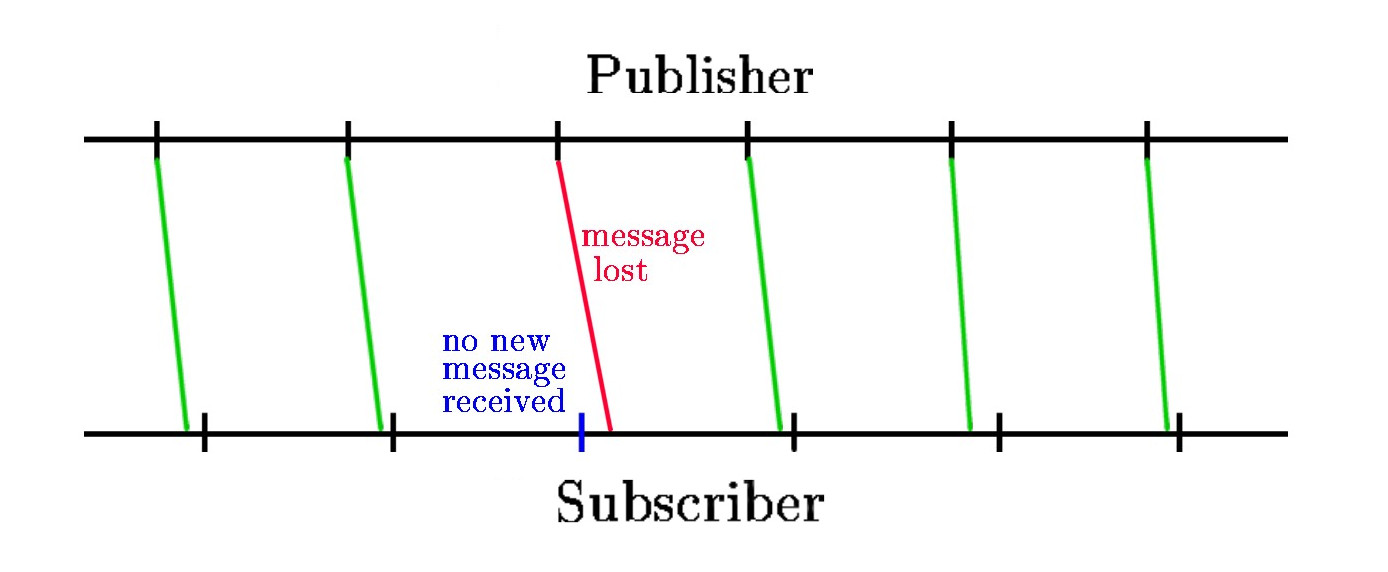
\includegraphics[height=6cm]{messages.jpg}
\caption{Uncertainty for the messaging system}\label{msg}
\end{center}
\end{figure}


In this report, we will establish a worst case scenario for this messaging system. For example, knowing that a node will always have available at least one message with a bounded age can be sufficient to assert a control loop maintains a state precisely enough around the desired value.
This can also be used for monitoring purposes: if a node detects a behavior outside this worst case scenario, it can raise an alert to a supervisor. By collecting these alerts, the supervisor could detect a compromised/crashed node, or a broken link, and decide how to fix the problem.

In Section 3, we give more details about the ROS architecture and the model used to represent it. In Section 4, we prove low-level properties for the messaging system. In sections 5 to 7, we give assurance claims for simple end-to-end properties. Section 5 proves that a basic control loop maintains a state around a set value. Sections 6 and 7 give two different models for obstacle avoidance.

\section{Related work}
\subsection{Assurance claims for quasi synchronous systems}

Synchronous models are easier to understand give more assurance properties, but keeping a distributed system synchronized is expensive in terms of computing time and exchanged messages, which leads to less efficient implementations.
Recent work proposes a method to translate a synchronous model to an equivalent Loosely Time-Triggered Architecture where nodes communicate through FIFOs with size 1 or 2 (see \cite{LTTA}).

However, a Finite FIFO Platform assumes the nodes skips a step when its output buffers are full. Used with a ROS architecture, this model is really vulnerable to attacks.
Assume an attacker compromised a node or created a useless one; then, by subscribing to many topics but refusing to read anything (to free space in the queues), it would cause the whole system to stop working.
Moreover, these proofs assume the communication channels preserves the order of messages, which is not necessarily the case in ROS.

\paragraph{ } The other approach is to prove properties directly for the quasi synchronous system, in order to use them for more complex applications. 
Then, such properties can be used for example to map synchronous arguments to quasi-synchronous systems (see \cite{Caspi}).
This work also describes a voting procedure in this case that asserts fault tolerance; that is, providing correct inputs even with faulty sensors.

Again, some assumptions are made that are few compatible with HACMS requirements. Considering that components have a periodic execution (with a period only known to be between some bounds) takes account of local clock uncertainty.
This is sufficient when the execution rate is reasonably slow, but with a higher rate, scheduling effects and variable computation time (depending on the input) should also be considered.
Also, while direct bus communication or shared memory ensure a message is available almost as soon as it is written, safety procedures in the underlying mailbox system in HACMS makes the transmission delay non negligible.



\subsection{Security and reliability in HACMS}

As part of the HACMS project, a \emph{Robot Architecture Description Language (RADL)} is being developed.
This language is used to describe the systems functional structure, that is nodes and topics are declared with their characteristics: rate, published and subscribed topics for nodes, message type for topics (see Figure~\ref{RADL}).
This allows two different tasks:

\begin{itemize}
\item checking architecture consistency: for example, message types must match for a topic and nodes publishing or subscribing to this topic.
This also allows to check various physical requirements. Among others: a physical device can be assigned to at most one node, or at most one node is allowed to publish on a given topic.

\item generating the running ROS configuration: ROS configuration files are automatically generated from the RADL according to the specified architecture.
A portion of node running code is also automatically generated. This includes initialization steps, and the few commands to read and check incoming messages at each periodic step.
The user has to write the so called \emph{step function}, that writes messages to published topics according to input values passed as arguments.
\end{itemize}

\begin{figure}[ht]
\begin{center}
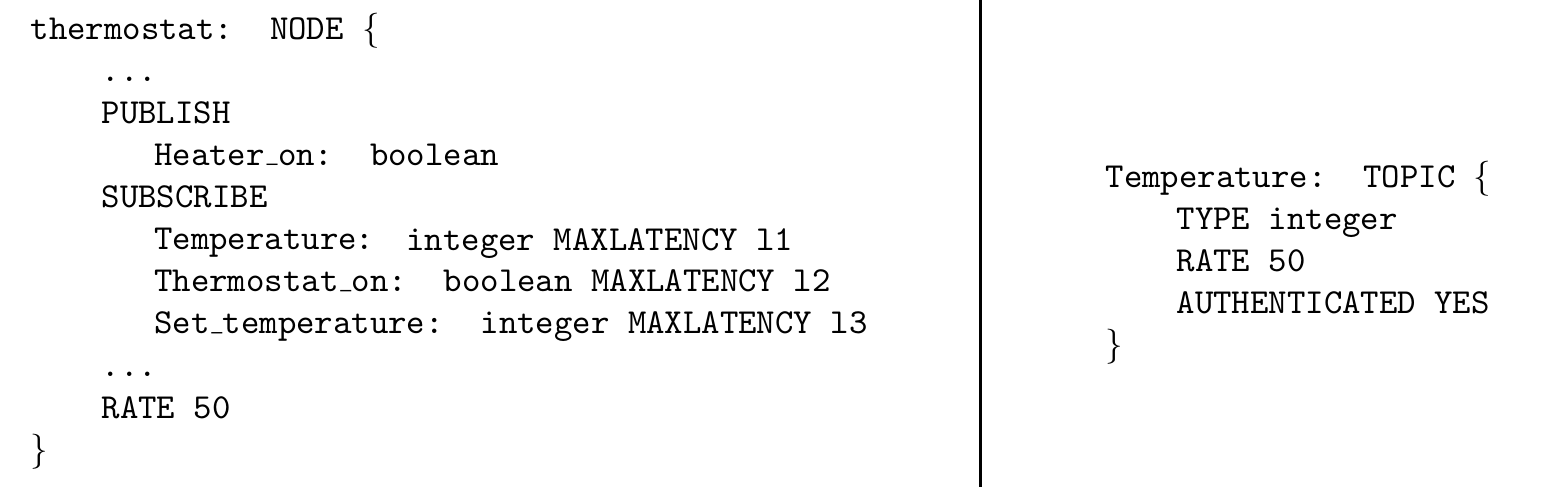
\includegraphics[width=15cm]{RADL.png}
\caption{A small RADL example}\label{RADL}
\end{center}
\end{figure}

Another interest is that the assurance properties from Section~\ref{prop} could be integrated to the code generated from RADL:
automatic checks could be added when reading input buffers, and when a node detects a behavior outside the framework given by these properties, it can report this error to a monitor and/or add a flag to sent messages to inform other affected nodes of this issue.
This allows attack detection as well as monitoring for software or hardware failure.

\paragraph{ }
Establishing assurance properties for a cyber-physical system means ensuring its behavior responds to the specification, even in presence of an attacker, and the HACMS project led to interesting work in this domain.

Security protocols and cryptography aren't enough to avoid a cyber-physical system being attacked: physical components can also being compromised.
An attacker can modify the physical environment around a sensor in order to inject malicious signal and to modify the system behavior.
A team from the University of Pennsylvania designed an algorithm to prevent such attacks (see \cite{StateEstimator}).
This algorithm ensures the state estimation error is bounded as soon as less than half the sensors are under attack (other sensors may experience a bounded noise).

This team also developed a cruise controller (see \cite{CruiseControl}) to control the speed of a vehicle. 
It ensures the difference between desired speed and actual speed is bounded after some time $T$, and this difference is exponentially decaying from time 0 to T.
The combination of the attack-resilient state estimator and the cruise controller ensures the vehicle travels at the speed set by the operator even when some sensors are compromised.



\subsection{The Prototype Verification System}

The \emph{Prototype Verification System (PVS)} is a specification language and theorem prover. The specification language uses typed higher-order logic.
Typing is needed to keep higher-order logic consistent, and also help to detect errors in the specification.
For instance, when the typechecker encounters an expression of the form \texttt{x/y}, it generates a \emph{Type Correctness Condition (TCC)}, that is a proof obligation to ensure \texttt{y} cannot be 0 in the current context.
Most of the time, automatic decision procedures manage to prove such TCCs, but sometimes, a user-made proof needs to be done\footnote{$ $
the rich type system in PVS, including constrained as well as uninterpreted subtyping, makes it non algorithmically decidable}
(and sometimes, the generated TCC is unprovable because of an error in the specification).
A more complete description of PVS can be found in the PVS user guide \cite{PVS:userguide}.

\begin{table}[ht]
\begin{center}
\begin{tabular}{|c||c|c|}
\hline
& \textbf{left} & \textbf{right} \\ \hline \hline
Axiom & 
\multicolumn{2}{|c|}{
\cell{\overline{\Gamma , A \vdash A , \Delta}}} \\ \hline

Bool. const. &
\cell{\overline{\Gamma , \texttt{FALSE} \vdash \Delta}}&
\cell{\overline{\Gamma \vdash \texttt{TRUE}, \Delta}} \\ \hline

Cut & 
\multicolumn{2}{|c|}{
\cell{\frac{\Gamma , A \vdash \Delta \qquad \Gamma \vdash A, \Delta}  {\Gamma \vdash \Delta }}} \\ \hline

$\neg$ &
\cell{\frac{\Gamma , \neg A \vdash \Delta}{\Gamma \vdash A , \Delta}}&
\cell{\frac{\Gamma \vdash \neg A , \Delta}{\Gamma , A \vdash \Delta}}\\ \hline

$\vee$ &
\cell{\frac{\Gamma , A \vdash \Delta \qquad \Gamma , B \vdash \Delta}  {\Gamma , A \vee B \vdash \Delta }}&
\cell{\frac{\Gamma \vdash A, B \Delta}  {\Gamma \vdash A \vee B, \Delta }} \\ \hline

$\wedge$ &
\cell{\frac{\Gamma , A, B \vdash \Delta}  {\Gamma, A \wedge B \vdash \Delta }}&
\cell{\frac{\Gamma \vdash A, \Delta \qquad \Gamma \vdash B, \Delta}  {\Gamma \vdash A \wedge B \Delta }} \\ \hline

$\implies$ &
\cell{\frac{\Gamma \vdash A, \Delta \qquad \Gamma , B \vdash \Delta}  {\Gamma , A \implies B \vdash \Delta }}&
\cell{\frac{\Gamma , A \vdash B \Delta}  {\Gamma \vdash A \implies B, \Delta }} \\ \hline

$\exists \: ^*$ &
\cell{\frac{\Gamma , A[\mathbf{x'}/x] \vdash \Delta }{\Gamma , \exists x . A \vdash \Delta}} &
\cell{\frac{\Gamma \vdash \Delta , A[\mathbf{t}/x]}{\Gamma \vdash \Delta , \exists x . A}} \\ \hline

$\forall \: ^*$ &
\cell{\frac{\Gamma, A[\mathbf{t}/x] \vdash \Delta}{\Gamma , \forall x. A \vdash \Delta}} &
\cell{\frac{\Gamma \vdash \Delta , A[\mathbf{x'}/x] }{\Gamma \vdash \Delta , \forall x . A}} \\ \hline

\multicolumn{3}{c}{
\begin{minipage}{13cm}\vspace{0.1cm}
$^*$ Quantifier elimination rules assume $\mathbf{x'}$ (in $\exists$~\emph{left} and $\forall$~\emph{right}) is a free variable that has no free occurrence in the sequent formulas.
Also, $\mathbf{t}$ (in $\exists$~\emph{right} and $\forall$~\emph{left}) is a term that doesn't contain a quantified variable appearing in any sub-formula of $A$.
\end{minipage}}

\end{tabular}
\end{center}

\caption{The (main) inference rules of sequent calculus}\label{LK}

\end{table}

The theorem prover is based on the inference rules of sequent calculus for propositional logic (see Table~\ref{LK}).
The prover is highly interactive and the user can choose which inference rule use at each branch of the proof tree until said branch leads to an axiom (which is a sequent calculus demonstration).
Sets of antecedent formulas $\Gamma$ are seen as a conjunction and consequent formulas $\Delta$ as a disjunction:
\[ \Gamma \vdash \Delta \quad \textrm{means} \quad \bigwedge \Gamma \implies \bigvee \Delta \]

The complete list of prover commands is available in the PVS prover guide \cite{PVS:prover}, but we present here the most useful. The \emph{Cut} rule with formula $A$ can be applied with the \texttt{case $A$} command.
\texttt{flatten} applies all possible simplifications for \emph{$\implies$ right, $\vee$ right, $\wedge$ left} and $\neg$.
\texttt{split} applies inference rule $\implies$\emph{left}, $\vee$ \emph{left} and $\wedge$ \emph{right} on a specified formula. 
\texttt{prop} is equivalent to applying \texttt{flatten} and \texttt{split} on every formula of the sequent (that can lead to a lot of subgoals).
Finally, \texttt{skolem} and \texttt{instantiate} are the quantifier elimination commands, for $\forall$ \emph{right}/ $\exists$ \emph{left} and $\forall$ \emph{left}/ $\exists$ \emph{right} respectively.

Some other useful commands are not associated to an inference rule but are shortcuts used in natural deduction.
\texttt{assert} is a light SMT (satisfiability modulo theories) solver that deals with equality theory, can simplify algebraic expressions over $\mathbb{R}$ up to a certain point and use some specific theorems.
\texttt{lemma \emph{thm}} adds the statement of theorem \texttt{\emph{thm}} to the set of antecedent formulas and \mbox{\texttt{expand \emph{name}}} replaces \texttt{\emph{name}} by its expanded definition.
\texttt{replace} uses an antecedent formula $\mathbf{t = t'}$ (where $\mathbf{t}$ and $\mathbf{t'}$ are terms) to replace $\mathbf{t}$ by $\mathbf{t'}$ in a given formula.


\paragraph{ } All results presented in Sections 4 to 6 have been formally proved using PVS. As we will see, proofs in Sections 5 and 6 are very similar.
These PVS proofs, currently \emph{hello world} examples, could become the base for automated proof procedures for such properties.




\section{The ROS architecture}
\subsection{Overview of ROS functioning}

The aim here is not to give a complete description of ROS (the interested reader could refer to ROS manuals, for example \cite{O'Kane201310}). However, a few notions about ROS abstraction could be needed to understand following sections.

The main purpose of ROS is to provide a framework for distributed computing. Rather than writing one complex program that runs the whole robot, designers prefer writing several simpler programs (potentially running on different computers) in charge of a specific task: 
one program that uses sensors to scan the environment, one responsible to interact with the operator, another one controlling the wheels and so on

Each of these programs is represented by a ROS \textit{node} that can send messages to other nodes.
\textit{Topics} are declared to group messages with the same function, and each node can be publisher or subscriber to one or more topics. 
The ROS master gives information to publishers (for example IP addresses or location of shared buffers), so when publishing a message on a topic, they can send messages to all subscribers to this topic.
Messages received by a subscriber are stored in a queue until they are computed. If the queue is full when a new message is received, the oldest message is thrown away. 



\subsection{Modeling assumptions}\label{ROSarch} 

\paragraph{Topic assumptions:}
To avoid jamming, we require at most one publisher per topic\footnote{$ $ no publisher on a topic generates a warning, but is considered non-critical}; this is secured in HACMS by message authentication and firewall rules.
For simplification purpose, we assume in this report that there is only one subscriber on each topic.
This assumption does not lead to a loss of generality: a topic with $n$ subscribers could be seen as $n$ topics with one subscriber.
Finally, we assume that the transmission delay for a given message is bounded.

Then, a topic can be characterized by two nodes (the publisher and the subscriber), the maximum transmission delay and the queue size for the subscriber.


\paragraph{Node assumptions:}
Nodes are discrete simple tasks executed regularly.
Each node is supposed to execute at a given frequency, but the actual rate may vary.
The execution could be non-periodic, but we assume that the time between two consecutive steps (or pseudo-period) is inside some known interval $[minT, maxT]$ with $minT > 0$.
The typical example is when the frequency is known with a certain drift $\rho$, and the actual instantaneous frequency is in $[(1-\rho).f, (1+\rho).f]$.

We also do the simplifying assumption that the task at each step is executed instantaneously. 
Actually, in the case of a node that is only a publisher (resp. subscriber)\footnote{$ $ for example a sensor (resp. actuator)}, the time of the execution event can be taken as the time when the node sends (resp. reads) the message, which are atomic operations.
In the case of an intermediate node, that is both subscriber and publisher on different topics, the computing duration between these two operations could just be added to the delay of the published topic.

Then a node can be characterized by the upper and lower bound for the pseudo-period between consecutive steps.


\paragraph{Notations:}
Events are described by functions from $\mathbb{N}$ (the system runs forever) to $\mathbb{R^+}$ that give the time when this event happens. For example, if $e$ is the function used to describe the executions of some node, $e(n)$ is the time when the nth execution occurs.

\begin{defin}\Thmname{Node execution}

Each node $N$ is defined by its minimal pseudo-period $minT(N)$ and maximal pseudo-period $maxT(N)$. 
Then an execution of $N$ is any function $e$ such that
\[ e(0) = 0 \quad \textrm{\emph{and}} \quad \forall n \in \mathbb{N}, \, 
e(n) + minT(N) \leq e(n+1) \leq e(n) + maxT(N) \]
\end{defin}

The assumption $e(0) = 0$ could seem too strong because it implies all nodes start exactly at the same time (which is quite unrealistic). First, having a common origin simplifies inductions, that are widely used in proofs. 
Second, we could prove that for any initial time shift $\Delta$, with an interval $[minT(N), maxT(N)]$ as small as desired, there exist executions for $N$ and $N'$ such that \mbox{$e(n) - e'(m) = \Delta$} for some $n$ and $m$.
This means that our model can be generalized to allow a time shift by assuming nodes $N$ and $N'$ send their default value (which is supposed to lead to a safe behavior) before periodic step $n$ and $m$.
An induction gives the result for more than 2 nodes:

The two nodes $N$ and $N'$ can be grouped into a single node $\hat{N}$ with period a common multiple of admissible periods for $N$ and $N'$: $\hat e(k) = k.T = e(n+ka) - e(n) = e'(m+kb) - e'(m)$.
Assume $N''$ has an initial time shift of $\Delta '$ with $N$. Apply previous result with $\hat N$ and $N''$ for a time shift of $\Delta ' - e(n)$: $e''(l) - \hat e(k) = \Delta ' - e(n)$. Then, $e''(l) - e(n+ka) = \Delta '$ and $e''(l) - e'(m+kb) = \Delta' - \Delta$ (initial time shift between $N'$ and $N''$).

\begin{defin}\Thmname{Message reception}\label{reception}

Let $T$ be a topic with a maximum transmission delay of $D$, and let $s$ be an execution of its publisher $S$ (associated to the event \emph{a message is sent}). 
A reception of these messages is any function $r$ such that
\[ \forall n \in \mathbb{N}, \, s(n) \leq r(n) \leq s(n) + D \quad 
\textrm{\emph{and}$\quad r$ is injective} \]
\end{defin}

The hypothesis that $r$ is injective means that two different messages cannot be received exactly at the same time. This is linked to hardware limitations, and is important to represent the queue: if messages $m$ and $n$ are received exactly at the same time, which one comes before the other in the queue?   

Note that this definition does not assume the channel conserves the order of messages. We could have $r(k) > r(k+1)$ and therefore, the message received just after message $n$ is not necessarily message $n+1$.
However, we can define a function $next$ such that there is no message received between $r(n)$ and $r(next(n))$.
Then the iterated function $Nth\_next$ is such that there is exactly $N-1$ messages received between $r(n)$ and $r(Nth\_next(N, n))$.
This means $next(n)$ is the message received just after $n$ is, and $Nth\_next(N, n)$ is the N'th message received after $n$ is.

\vbox{
\begin{defin}\Thmname{Processed message}

Let $T$ a topic with a subscribers queue size of $L$. Let $s$ and $c$ be an execution of its publisher and subscriber and $r$ be a reception of sent messages.

By definition, we have $\big |\{k\, | \, r(n) \leq r(k) < r(Nth\_next(L, n))\} \big | = L$. Then, message $n$ is in the queue at time $t$ iff \footnote{$ $ Actually, depending on the implementation, the message could be removed from the queue during a computation, but before $r(Nth\_next(L, n))$.
This does not affect the definition.}
 \mbox{$r(n) \leq t < r(Nth\_next(L, n))$}
 
A message $n$ is said to be \emph{processed} if and only if 
\[ \exists k \in \mathbb{N}, \quad r(n) \leq c(k) < r(Nth\_next(L, n)) \]
\end{defin}
}

The message is said to be \emph{lost} or \emph{dropped} otherwise



\section{Low-level messaging system}\label{prop}
In this section, we consider a topic $T$, characterized by a publisher $P$, a subscriber $S$, a maximum transmission delay $D$, and a queue length $L$.

For $n \in \mathbb{N}$, we note $s(n)$ and $r(n)$ respectively the time when the n'th message is sent and received. We also note $c(n)$ the time when the subscriber executes its n'th computation.

\subsection{Latency}

For a processed message, we define its latency as the duration between the time it is sent and the time it is computed for the first time (see Figure~\ref{latency}):

\begin{figure}[h]
\begin{center}
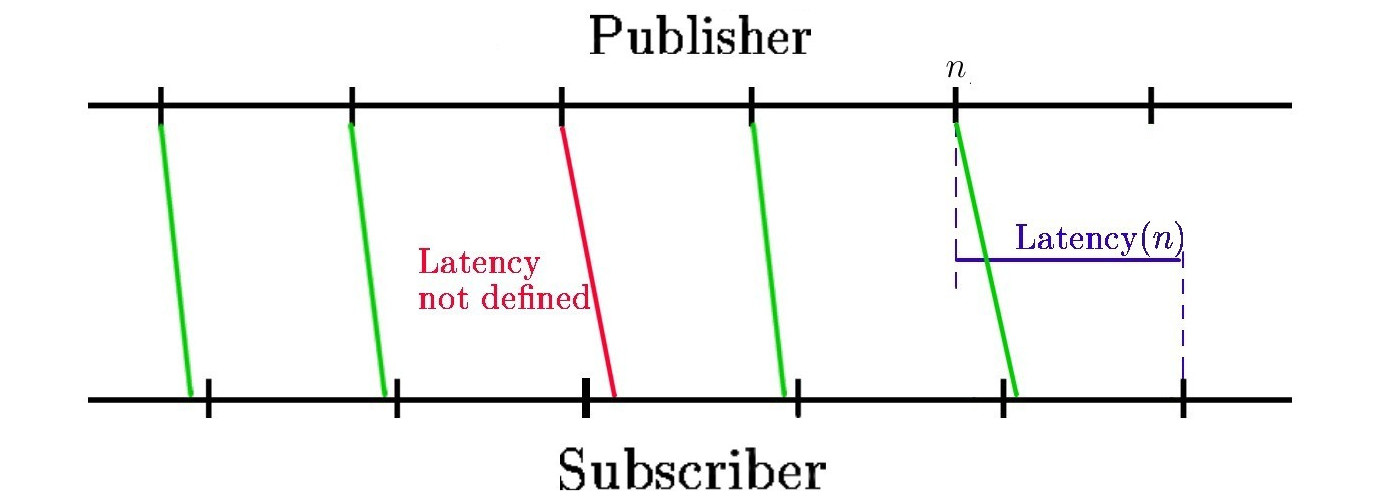
\includegraphics[height=5cm]{latency.jpg}
\caption{Latency definition}\label{latency}
\end{center}
\end{figure}

\begin{defin} \Thmname{Latency}
\[ Latency(n) = c \Big ( min(\{k \in \mathbb{N} | r(n) \leq c(k)\}) \Big ) - s(n) \]
\end{defin}

Since $\forall k, c(k + 1) \leq c(k) + maxT(S)$, we have
$c \big ( min(\{k \in \mathbb{N} | r(n) \leq c(k)\}) \big ) - r(n) \leq maxT(S)$. Therefore,
\begin{thm}\Thmname{Latency bound}
\[ Latency(n) \leq maxT(S) + D \]
\end{thm}

The latency is only defined for a processed message, so this gives little information for assurance properties. However, it can be used to detect a clock failure or a certain type of attack: 
assume for example that the subscriber reads a new message, but the delay since the messages timestamps exceed the latency bound. 
It could be that the clock of one of the nodes drifted significantly from real time, or it may mean that the message had been recorded and was resent later by an attacker.



\subsection{Overtaking}

The model defined in section \ref{ROSarch}, allows an older message to be delivered after a more recent one. We may want to avoid this even if the mailbox system alone doesn't assert that this property holds.
We give here a simple condition that asserts that messages are received in the order they are sent. 

Avoiding overtaking can yield better bounds in some cases to assert other properties are satisfied. By choosing good nodes parameters, a developer can also secure the order of received messages and rely on this to prove correctness of an application.

We have $r(n) \leq s(n) + D$, $s(n) + minT(P) \leq s(n + 1)$ and $s(n + 1) \leq r(n + 1)$. Hence the following theorem:

\begin{thm} \Thmname{Overtaking}
\[ D < minT(P) \quad \implies \quad \forall n \in \mathbb N, \quad r(n) < r(n + 1)\]
\end{thm}


\subsection{Number of lost messages}

As we saw before, messages can be overwritten in the queue before they are actually computed by the subscriber, which means these messages are never processed. However, we can ensure the subscriber does not miss too many consecutive messages

\subsubsection[Consecutive lost messages]{Upper bound for the number of consecutive lost messages}

\begin{defin}\label{consec}
\Thmname{Consecutive lost messages}\\
Formally, we can define the property "the subscriber never misses N consecutive messages" by
\[ \forall k \in \mathbb{N}, \exists l < N, \quad \textrm{\emph{message $k + l$ is processed}}   \]
\end{defin}

First, we have this fundamental lemma:
\begin{lem}\label{existsProcess}
If $c(n) \geq t + D + maxT(P)$, there exists a message $k$ with $t < r(k) \leq c(n)$ that is processed.
\end{lem}

\begin{proof}
$r(0) \leq D < c(n)$. Let $m$ be the maximum of the $l \in \mathbb{N}$ such that $r(l) \leq c(n)$. Since $r(m + 1) > c(n)$, we have $t < r(m) \leq c(n)$.

The set $S = \{l \in \mathbb{N}, t < r(l) \leq c(n)\}$ is finite and nonempty. There exists a $k \in S$ such that $\forall l \in S, r(l) \leq r(k)$. By construction, such a $k$ solves the problem because no message is received between $r(k)$ and the next execution of the subscriber.
\end{proof}

Basic inequality reasoning give this result:

\begin{lem}\label{order_received}
\[ r(m) > s(n) + D - minT(P) \implies n \leq m \]
\[ r(m) < s(n) + minT(P) \implies m \leq n\]
\end{lem}

\begin{thm}\label{clm}\Thmname{Consecutive lost messages}

If $N.minT(P) > 2.D + maxT(S) + maxT(P) - minT(P)$, then the subscriber never misses $N$ consecutive messages.
\end{thm}

\begin{proof}
According to definition~\ref{consec}, given $k \in \mathbb N$, we prove there exists an $l < N$ such that message $k + l$ is processed.

The subscriber executes at least once in every interval of time of length $maxT(S)$. In particular, 
\[ \exists n \in \mathbb N, \quad 
\left\{
\begin{array}{l}
s(k) + 2.D + maxT(P) - minT(P) < c(n) \\
c(n) \leq s(k) + 2.D + maxT(P) - minT(P) + maxT(S)
\end{array} \right. \]

Lemma \ref{existsProcess} gives $\exists l \in \mathbb{N}, s(k) + D - minT(P) < r(l) \leq c(n)$ such that the message $l$ is processed. Since $s(k + N - 1) \geq (N-1) . minT(P)$, with the given condition on $N$, $c(n) < s(k + N - 1) + minT(P)$.

With lemma \ref{order_received}, we have $k \leq l \leq k + N - 1$, and $l$ is processed by construction.
\end{proof}

\paragraph{Case without overtaking :} Assume now that $\forall k \in \mathbb N,\,\, r(k) < r(k + 1)$. In that case, with $m = max({k \in nat, r(k) \leq c(n)})$ we have $r(k) \leq c(n) \implies r(k) \leq r(m)$ which ensures message $m$ is processed.

With $N.minT(P) > D + maxT(S)$, we have $\exists n \in \mathbb N, s(k) + D \leq c(n) < s(k + N)$, then $r(k) \leq c(n) < r(k + N)$. We deduce message $m$ is processed with $k \leq m < k + N$.

\begin{thm}\label{clm2}\Thmname{Consecutive lost messages -- no overtaking}

Assume $N.minT(P) > D + maxT(S)$ and $\forall k \in \mathbb{N},\,\, r(k) < r(k + 1)$. Then the subscriber never misses $N$ consecutive messages.
\end{thm}


\subsubsection{Influence of the queue length}

As one can expect, increasing the message queue size leads to a lower message loss rate. For more comprehension, we first prove this in the case without overtaking. 
Then, we give an idea of the proof in the general case.

Assume we have $\forall k \in \mathbb{N},\,\, r(k) < r(k + 1)$ and we never drop $N$ ($N > 1$) messages with a queue length of $L$. Given $k \in \mathbb N$, there exists $l < N$ such that message $k + l$ is processed. 
If $l < N - 1$, the result is proved. If $l = N - 1$, it means the message $k + N - 1$ was in the queue when some computation $c(n)$ occurred.
With a queue length of $L + 1$, the message $k + N - 2$ was in the queue when $c(n)$ occurred, which means it was processed.

\paragraph{ }
In the general case, we assume the property "never miss $N$ consecutive messages" holds whatever $r$ is as soon as the constraints with $s$ and $D$ are respected (theorem \ref{clm} gives this assurance).
Like in the previous proof, we assume $k + N - 1$ is processed and none of the $k + l$ with $l < N - 1$ is. 
Among non-processed messages received before $r(k + N - 1)$, let $m$ be the one received last. With a queue length of $L + 1$, $m$ is processed with the same argument as before. The difficult part is to prove that this $m$ exists and must be one of the $k + l$, $l < N - 1$.
For this, we construct an other $r'$, consistent with the constraints on $s$ and $D$ but with $N$ consecutive messages lost (which is a contradiction).

Assume that none of the $k+l$ verifies $r(k+l) < r(k+N -1)$. Let $r'$ be a new reception sequence where reception of message $k+N-1$ is delayed to $r(k) + \varepsilon$ (see Figure~\ref{contr}.a),
where $\varepsilon$ is small enough to ensure $r'$ verifies constraints of definition~\ref{reception} and that no message is received between $r'(k)$ and $r'(k+N-1)$.
In this case, messages $k$ to $k+N-2$ are lost because messages that overwrote them with reception $r$ still do with reception $r'$, and message $k+N-1$ is lost because it is received between message $k$ (that is lost) and the next processed message.
This proves $m$ exists and verifies $r(k+l) \leq r(m) < r(k+N-1)$ for some $l$.

Assume $m > k+N-1$. Let $r'$ be the reception sequence where reception of messages $m$ and $k+N-1$ are switched (no change for other messages; see Figure~\ref{contr}.b). $m$ was lost with $r$ means $k+N-1$ is lost with $r'$. Again, messages $k$ to $k+N-1$ are lost with $r'$.

Assume $m < k-1$ (case $m=k-1$ is impossible: $k-1$ must be processed since none of the $k,\dots,k+N-2$ is). If $r(k-1) < r(m)$, switching reception of $k-1$ and $m$ (see Figure~\ref{contr}.c) gives a contradiction with the same argument as previously.
Otherwise, we consider the reception sequence $r'$ where reception of message $k-1$ is anticipated to $r(m)-\varepsilon$. Then, messages $k-1$ to $k+N-2$ are lost (see Figure~\ref{contr}.d).

\begin{figure}[h]
\begin{center}
a) Case $\forall l \in [0, N-2], r(k + l) > r(k+N-1)$ (includes the case where $m$ does not exist)\\
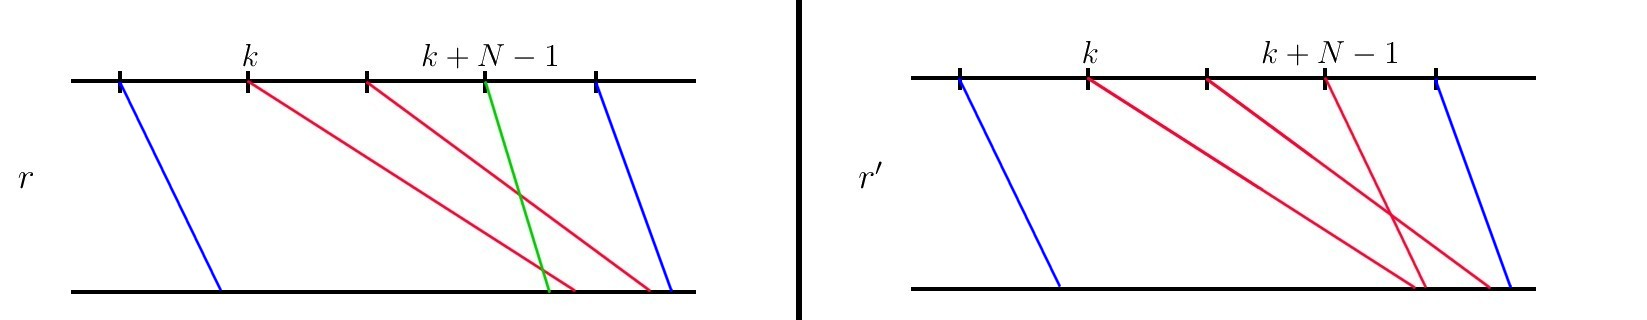
\includegraphics[width=16cm]{contr1.jpg}\\
b) Case $m > k+N-1$\\
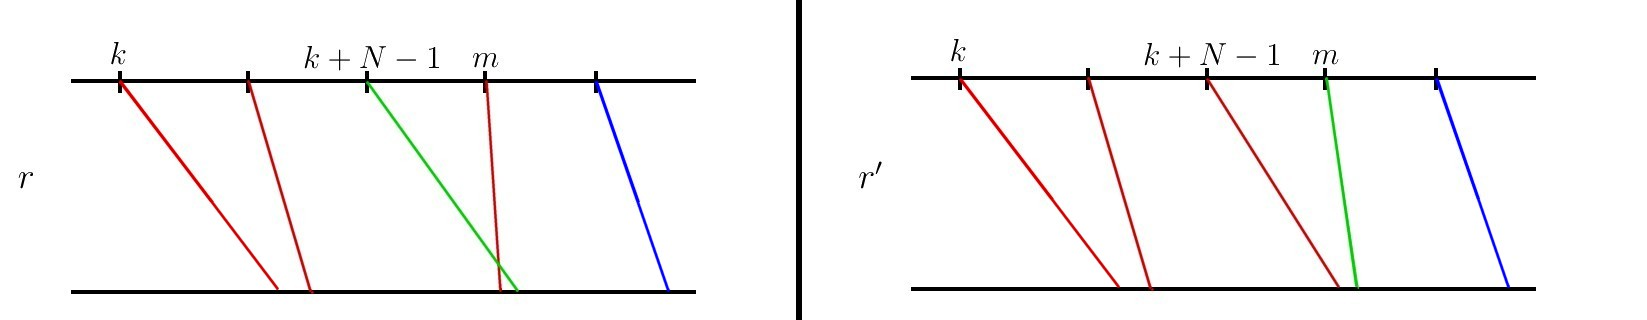
\includegraphics[width=16cm]{contr2.jpg}\\
c) Case $m < k-1$ and $r(m) > r(k-1)$\\
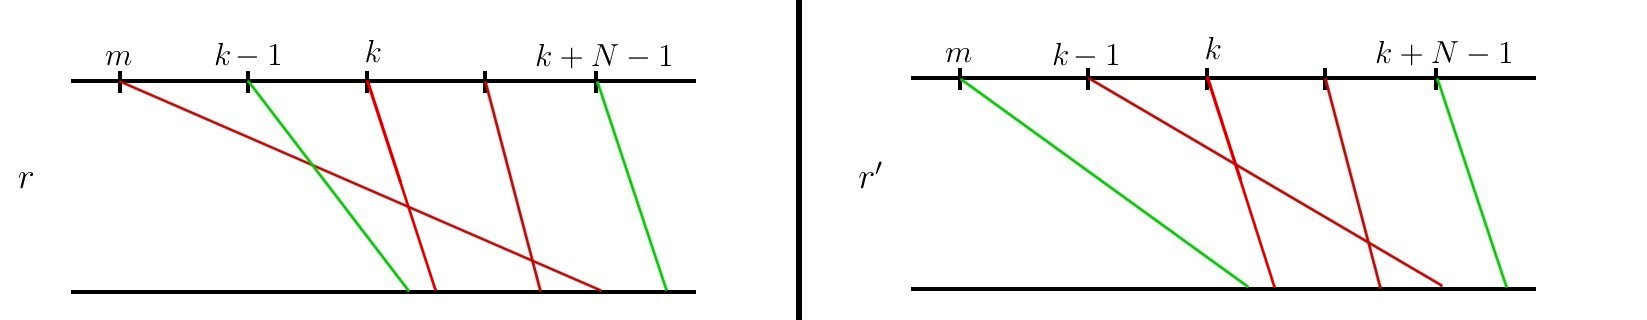
\includegraphics[width=16cm]{contr3.jpg}\\
d) Case $m < k-1$ and $r(m) < r(k-1)$\\
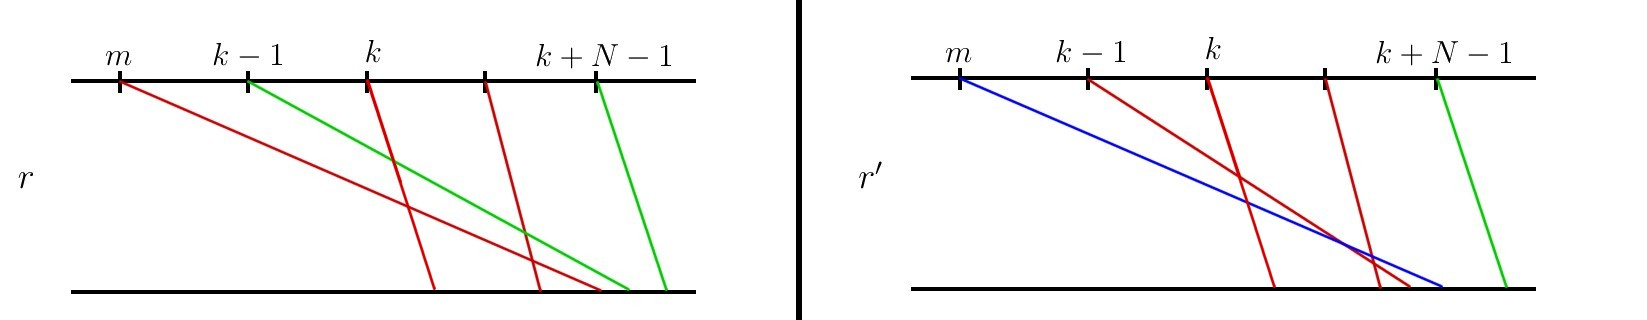
\includegraphics[width=16cm]{contr4.jpg}\\
(green: processed -- red: lost -- blue: status unknown/irrelevant)
\caption{Getting contradictions}\label{contr}
\end{center}
\end{figure}

\paragraph{ }By a simple induction, we then get the following result:

\begin{thm} 
Let $N$ satisfies conditions of either theorem~\ref{clm} or theorem~\ref{clm2}. Let $m < N$ and assume $L > m$. Then the subscriber never miss $N - m$ consecutive messages.

In particular, if $L \geq N$, no message is lost.
\end{thm} 

\subsection{Age of processed messages}

In this section, we prove that at each computation, the subscriber gets (from a newly received message or with a backup from previous computation) a reasonably recent message.

This is essentially a bound on the age of processed messages that will be used in next sections to prove end-to-end properties. It is also helpful to detect errors: when the latest available message to the subscriber is older than the bound, it can raise a timeout flag. By collecting these flags, a monitor could guess whether the publisher node crashed or there is a network failure.

\subsubsection{Definition and basic properties}

The aim is to model the following behavior (see Figure~\ref{age}):
 At each computation, if messages are available in the queue, the node chooses the most recent one and saves it to give a backup solution for next computation. 
If not, it uses the backup given by previous step (while no message has been received, and no backup is available, a default value -- set at initialization time -- is used)

\begin{figure}[h]
\begin{center}
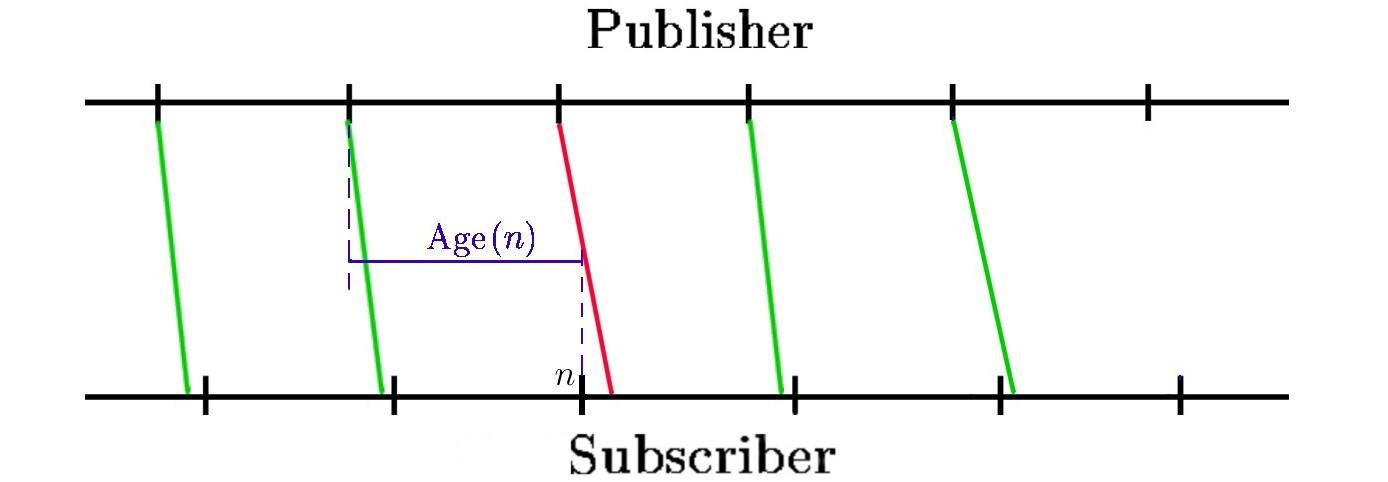
\includegraphics[height=5cm]{age.jpg}
\caption{Age definition}\label{age}
\end{center}
\end{figure}


\vbox{
\begin{defin}\label{ageDef}\Thmname{Age for the most recent available message}

For $n \neq 0$, we define the (finite, but maybe empty) set of messages computed at step n by
\[PL(n) = \big \{k \in \mathbb{N}, c(n - 1) < r(k) \leq c(n) 
\wedge \textrm{\emph{message $k$ is processed}} \big \}\]

Then, the age of the most recent available message can be defined by the recursive function \\
\emph{\texttt{Age($n$) = \{\\
\indent if $n=0$ then 0 \\
\indent else \{if $PL(n) = \emptyset$\\
\indent\indent then \{Age($n - 1$)$ + c(n) - c(n-1)$\}\\
\indent\indent else \{$c(n) - s(max(PL(n))$\}\\
\}\}
}}
\end{defin}
}

\vbox{
\begin{lem}\label{ageLem}
A simple induction over $n$ gives \texttt{\emph{Age}($n$)}$\leq c(n)$. 

Also, with the same argument as in the proof of lemma~\ref{existsProcess}, we have:
\[PL(n) = \emptyset \,\, \Longleftrightarrow \,\, 
\{k \in \mathbb{N}, c(n - 1) < r(k) \leq c(n)\} = \emptyset
\]
\end{lem}
}

\subsubsection{Upper bound in worst case scenario}

\begin{thm}\label{maxAge}\Thmname{Age bound}
\[ \texttt{\emph{Age($n$)}} < 2.D + maxT(P) \]
\end{thm}

\begin{proof}
First, we see by a simple induction over n that:
\[r(k) \leq c(n) \implies \texttt{Age($n$)} \leq c(n) - r(k) + D\]
(if $PL(n) = \emptyset$, lemma~\ref{ageLem} gives $r(k) \leq c(n-1)$. Otherwise, using the definition of a processed message, we either have $r(k) \leq r(max(PL(n)))$ or $k \leq max(PL(n))$. In both cases, \mbox{$s(max(PL(n))) \geq r(k) - D$})

In the case $c(n) \leq D + maxT(P)$, lemma~\ref{ageLem} gives the result. Otherwise, by lemma~\ref{existsProcess}, there exists a message $k$ such that $c(n) - D - maxT(P) < r(k) \leq c(n)$, which proves the theorem with the property above.
\end{proof} 

When messages are delivered in the same order they were sent, we get a better bound:

\begin{thm}\label{maxAge2}\Thmname{Age bound -- no overtaking}
\[ \forall k \in \mathbb{N},\,\, r(k) < r(k+1) \quad \implies \quad
\texttt{\emph{Age($n$)}} < D + maxT(P) \]
\end{thm}

\begin{proof}
When no overtaking is possible, the message $m(n) = max(\{k\in \mathbb{N},\, r(k) \leq c(n)\})$ (assuming the considered set is non empty) is processed. 

Since $r(m(n)+1) \leq s(m(n)) + D + maxT(P)$, we have 
\[ c(n) - D -maxT(P) < s(m(n)) \leq c(n) \]

$r(m(n)) \leq c(n-1) \implies m(n) = m(n-1)$. Therefore, we get by induction 
\[ \texttt{Age($n$)} = 
\left\{ \begin{array}{ll}
c(n) - m(n) &\textrm{ if $ r(0) \leq c(n)$}\\
c(n) &\textrm{ if $ r(0) > c(n)$, which means $c(n) < D$}
\end{array}\right.
\]
\end{proof}




\section{Assurance claim for the plant controller}
\subsection{Physical model and hypothesis}

In this section, we look at a control loop with a plant (external state we wish to maintain), a sensor which measures the plant state, a controller and an actuator. The actuator can be \textit{on} or \textit{off}, which gives two different progression modes for the plant. 
The controller sets the actuator \textit{on} or \textit{off} according to the input from the sensor and the settings from an operator.
Said operator can decide to enable or disable control, and can set preferences for the value to maintain the state around. This is summarized in Figure~\ref{plant}. For now, we assume the operator enables the control (no interest otherwise) and doesn't change the settings.

\begin{figure}[ht]
\begin{center}
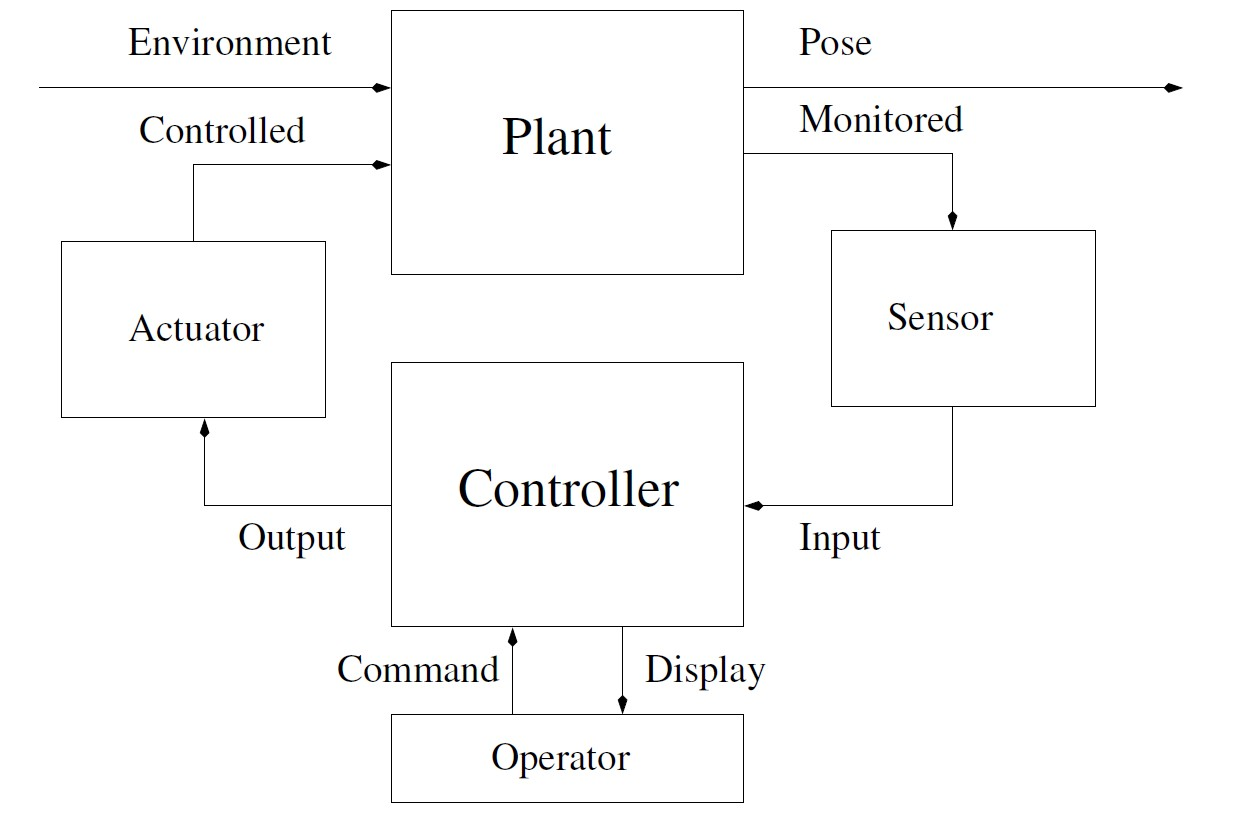
\includegraphics[height=7cm]{plant_controller.jpg}
\caption{The plant controller model}\label{plant}
\end{center}
\end{figure}


We consider the plant state as a real function of the time. The aim for the plant controller is to bring this state between two bounds and to maintain it there. A first example could be a thermostat: we want to maintain a room temperature around a comfortable value by switching a heater \textit{on/off} when needed.
We can also imagine maintaining a correct speed for a vehicle by giving or not power to the engine.

For better comprehension, we will use the vocabulary of the thermostat example in the rest of this section (but the model is actually more general).
We name $\theta (t)$ the temperature at time $t$, and $\tau$ and $\Gamma$ the upper and lower bounds in which we want to maintain the temperature.
We consider that the room leaks energy, and that the heater is powerful enough to increase the room temperature. Typically, while the heater is off, the room temperature decreases with a rate of at most $\mu$, and it increases with a rate of at least $\nu - \mu$ ($\nu > \mu$) while the heater is on. More precisely, considering the temperature is piecewise differentiable,

\[ \left\{ \begin{array}{rcccccll}
0 < & \nu - \mu & < & \dot \theta & < & \Omega   &    &\textrm{If the heater is \textit{on}}\\
    &- \mu    &   < & \dot \theta & < & - \omega & < 0 & \textrm{If the heater is \textit{off}}
\end{array}\right. \]

Assuming the outside temperature is lower than the inside temperature (who needs a heater otherwise?), this model is quite realistic, at least in a reasonable inside temperature range.

To represent real-life devices, we allow the sensor to be slightly inaccurate. Therefore, if the actual temperature is $\theta$, the sensed temperature will be $\sigma$ with 
$\theta - \epsilon \leq \sigma \leq \theta + \epsilon $



\subsection{Controller strategy}

The intuitive way is to set the heater \textit{on} when the temperature is too low, and set it \textit{off} when the temperature is too high. We define two trigger temperatures $\Delta_1$ and $\Delta_2$ with $\tau < \Delta_1 \leq \Delta_2 < \Gamma$. 
When the measured temperature is below $\Delta_1$, the controller switches the heater to \textit{on}, and 
when the measured temperature is above $\Delta_2$, the controller switches the heater to \textit{off}. 
The behavior when the temperature is between $\Delta_1$ and $\Delta_2$ doesn't really matter, so we decide for example to resend previous command.

Of course, we do not use $\tau$ and $\Gamma$ as triggers because of the sensor inaccuracy and because of the potential message latency (see Figure~\ref{trig}).

\begin{figure}
\begin{center}
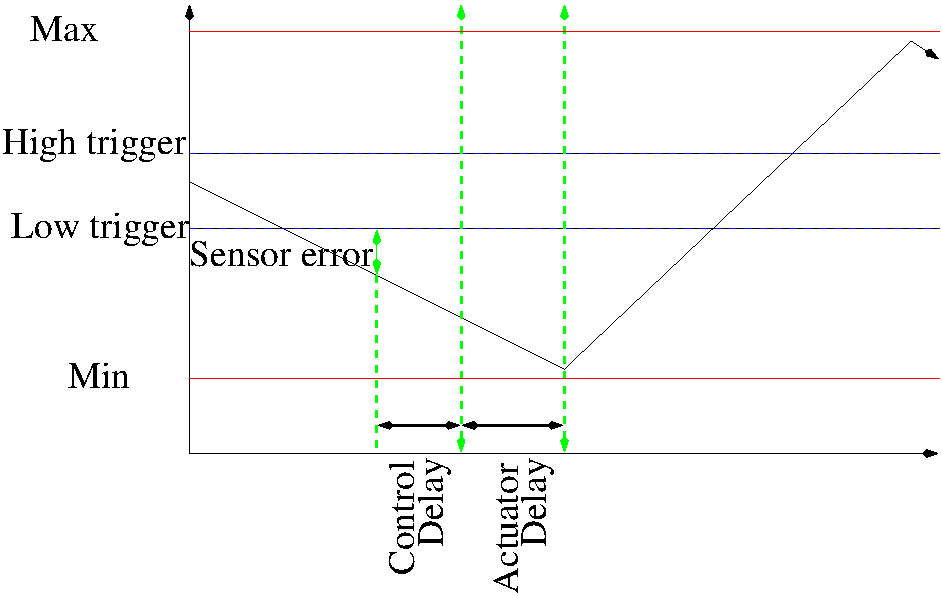
\includegraphics[height=7cm]{thermobehavior.pdf}
\caption{Effect of sensor inaccuracy and control and actuation latencies}\label{trig}
\end{center}
\end{figure}

This strategy could be implemented as follows: The controller keeps a binary setting, initialized to some default value. At each step, if a new message have been received, the controller chooses the most recent one and look at the sensed temperature $\sigma$ inside.
If $\sigma < \Delta_1$, the setting is turned to \textit{on}. If $\sigma > \Delta_2$, the setting is set to \textit{off}. Otherwise, no change is applied to the setting. After this test, the current setting is sent to the actuator.
(using the previous setting also in case no new message have been received is equivalent to use a backup from the previous computation)


\subsection{Correctness proof}\label{MAdef}

To prove correctness of the system, we need to apply this physical model to our logical architecture.
We name $S$, $C$ and $A$ the nodes for the sensor, the controller and the actuator respectively.
We note $s(n)$, $c(n)$ and $a(n)$ the time when their respective nth computation occurs. Let $Input$ and $Output$ be the topics for the sensed temperature and control commands respectively 
(that is, $S$ publishes to $Input$, $C$ subscribes to $Input$ and publish to $Output$, and $A$ subscribes to $Output$). 
Let finally $r_1(n)$ and $r_2(n)$ be the times when the nth message in these topics is delivered.

\vbox{
\begin{defin}\Thmname{Plant controller characteristic time}

For a topic $T$, we note $MA(T)$ some bound for the age of latest available message\footnotemark at each step (given for example by theorem~\ref{maxAge} or theorem~\ref{maxAge2}).

The characteristic time for the plant controller is the quantity
\[ \lambda = MA(Input) + MA(Output) + maxT(A)\]
\end{defin}
}
\footnotetext{$ $ see definition~\ref{ageDef}}

\vbox{
\begin{thm}\Thmname{State stability}\label{control}

Assume $\theta(t) \geq \Delta_1 - \epsilon \geq \tau + \lambda.\mu$ for some time $t$. Then, $\theta(t)$ never drops below $\tau$ after that: \mbox{$\forall t' \geq t, \, \theta(t') > \tau$}

Symmetrically, assume $\theta(t) \leq \Delta_2 + \epsilon\leq \Gamma - \lambda.\Omega$ for some time $t$. Then, $\theta(t)$ never becomes above $\Gamma$ after that: \mbox{$\forall t' \geq t, \, \theta(t') < \Gamma$}
\end{thm}
}

\begin{proof}
Let $t' \leq t$ and $g = glb(\{u \in \mathbb{R}, \, t \leq u \leq t' \textrm{ and } \theta(u) \leq \Delta_1 - \epsilon\})$. By definition, $\theta(g) = \Delta_1 - \epsilon$ and $g < u \leq t' \implies \theta(u) < \Delta_1 - \epsilon$.

Given $\dot{\theta} > -\mu$, if $t' \leq g + \lambda$, the result is proved. Otherwise, we prove $\theta(t') \geq \theta(g + \lambda) > \tau$, because the actuator is always \textit{on} in the time  interval $[g + \lambda, t']$:

Let $u \geq g + \lambda$. The actuator state at time $u$ was set at the latest computation $a(n)$ of $A$.
$a(n+1) \leq a(n) + maxT(A)$ so we have $a(n) > g + MA(Input) + MA(Output)$.
The corresponding command from the thermostat was issued at some $c(k)$ and by definition of $MA(Output)$,
we have $c(k) > g + MA(Input)$. This command was computed by comparing a measured temperature with $\Delta_1$ and $\Delta_2$.
Let $s(l)$ the execution that measured this temperature. We have $s(l) > g$ (by definition of $MA(Input)$), which means $\theta(s(l)) < \Delta_1 - \epsilon$.
Therefore, the sensed temperature was \mbox{$\sigma(s(l)) < \Delta_1$}
\end{proof}

\begin{thm}\Thmname{State convergence}

Assume $\theta(t) < \Delta_1 - \epsilon$. Then we have $\theta(t') \geq \Delta_1 - \epsilon$ for some $t'$ with 
\[t' < t + \lambda + \frac {\Delta_1 - \epsilon - \theta(t) + \lambda.\mu} {\nu - \mu} \]

Symmetrically, assume $\theta(t) > \Delta_2 + \epsilon$. Then we have $\theta(t') \leq \Delta_2 + \epsilon$ for some $t'$ with
\[t' < t + \lambda + \frac {\theta(t) + \lambda.\Omega - \Delta_2 - \epsilon} {\omega} \]
\end{thm}

\begin{proof}
Assume for all $u$ with $t \leq u \leq T = t + \lambda + \frac {\Delta_1 - \epsilon - \theta(t) + \lambda.\mu} {\nu - \mu}$, we have $\theta(u) < \Delta_1 - \epsilon$.
With the same argument as in previous theorem, the heater is always on in the time interval $[t + \lambda, T]$. 

During this interval, the temperature increases at a minimum rate of $\nu - \mu$. Therefore, $\theta(T) > \theta(t + \lambda) + (\Delta_1 - \epsilon - \theta(t) + \lambda.\mu)$. But $\theta(t + \lambda) > \theta(t) - \lambda.\mu$, which leads to a contradiction
\end{proof}








\section{Obstacle avoidance with dynamic window algorithm}
There exist proved obstacle avoidance procedures based on a \emph{dynamic window} algorithm (see, e.g. \cite{Mitsch-RSS-13}).
Among reachable speeds from the current state within some small delay (the \emph{dynamic window}), the system choses one that is both optimized in the sense of an objective function, and allows the vehicle to stop before hitting an obstacle.
In this section, we apply this strategy to our system and we prove that it effectively allows to stop soon enough.

\subsection{Objectives}

We consider the worst possible case that the vehicle runs in straight line directly directed to a fixed obstacle. We assume a sensor gives distance to the obstacle and vehicle speed up to a certain accuracy.
When the measured distance is too low, the controller sends an \emph{emergency stop} command that should bring the vehicle to full stop without hitting the obstacle.

The mechanical properties of the system give a maximum acceleration $A$ and a braking power $b$; such that $-b \leq \dot v \leq A$ and, while the brakes are used, $\dot v = -b$ or $v = 0 \wedge \dot v = 0$.
Let $\varepsilon$ be an upper bound for the control loop time interval and $D$ a minimal distance we want to keep from the obstacle.
Then, as said in \cite{Mitsch-RSS-13}, for a velocity $v$, a distance less than $\frac {v^2} {2b} + \left(\frac A b + 1 \right) \left( \frac A 2 \varepsilon^2 + \varepsilon.v\right) + D$ should cause the vehicle to brake.

Like in previous section, we use $\varepsilon = MA(Input) + MA(Output) + MaxT(A)$.

\subsection{Correctness proof}

Because of the sensor accuracy $\epsilon_d$ on the distance and $\epsilon_v$ on the velocity, the controller sends the \emph{emergency stop} command as soon as the measured distance $d_m$ and velocity $v_m$ verify
\[ d_m - \epsilon_d \leq \frac {(v_m + \epsilon_v)^2} {2b} + \left(\frac A b + 1 \right) \left( \frac A 2 \varepsilon^2 + \varepsilon.(v_m + \epsilon_v)\right) + D\]
This way, if the actual distance is less than $\frac {v^2} {2b} + \left(\frac A b + 1 \right) \left( \frac A 2 \varepsilon^2 + \varepsilon.v\right) + D$, this command is sent even with sensor inaccuracy.

If the latest message available to the actuator contains the \emph{emergency stop} flag, it activates the brakes. Otherwise, it keeps a standard behavior (keep the same speed, respond to operator commands~\dots).
This allows for example to activate the brakes, and release them at the next step because the speed decreased, or because of different sensor errors (first, the distance was underestimated and the speed overestimated, then the contrary happened).

\begin{thm}\Thmname{Obstacle avoidance}

Assume at time $t$, the vehicle is in a safe situation: $d(t) \geq \frac {v(t)^2} {2b} + \left(\frac A b + 1 \right) \left( \frac A 2 \varepsilon^2 + \varepsilon.v(t)\right) + D$.
Then the vehicle stops with a minimum distance to the obstacle: $\forall s, \, d(s) \geq D$
\end{thm}

\begin{proof}
For simpler notation, let $\delta(v) = \frac {v(t)^2} {2b} + \left(\frac A b + 1 \right) \left( \frac A 2 \varepsilon^2 + \varepsilon.v(t)\right) + D$ and assume $d(s) < \delta(v(s))$ (the result is already proved otherwise). Let $l = lub(\{r \in [t, s], \, d(r) \geq \delta(v(r))\})$.

We have $d(l) = \delta(v(l)) \geq D + \frac A 2 \varepsilon^2 + \varepsilon.v(l)$, which is the maximum distance the vehicle can travel during $\varepsilon$. Then, if $s \leq l + \varepsilon$, the result is also proved.
Otherwise, with the same argument as in the proof of Theorem~\ref{control}, the brakes are always activated in $[l + \varepsilon, s]$. During this time, the vehicle travels at most (if the vehicle has not come to full stop yet) the distance needed to stop completely, which is 
\[\frac {v(l + \varepsilon)^2} {2b} \leq \frac{(v(l) + A.\varepsilon)^2}{2b}\]
\end{proof}

\section{Alternative strategy for obstacle avoidance}
In this section, we describe a different strategy that aims to avoid the following too restrictive behavior: the strategy used in \cite{Mitsch-RSS-13} only reason about distance to the obstacle. This means that a straight line trajectory should keep a uselessly large distance to obstacles on the side (see Figure~\ref{OA}).

Again, we consider a moving vehicle and we add an interaction with an operator. The operator would like to move the vehicle by giving driving directions, that is, a desired instantaneous speed, and these directions must be rejected if they make the vehicle run into the obstacle.
This is because the operator may not have paid attention, or because the communication link may be compromised by an attacker.

\begin{figure}[ht]
\begin{center}
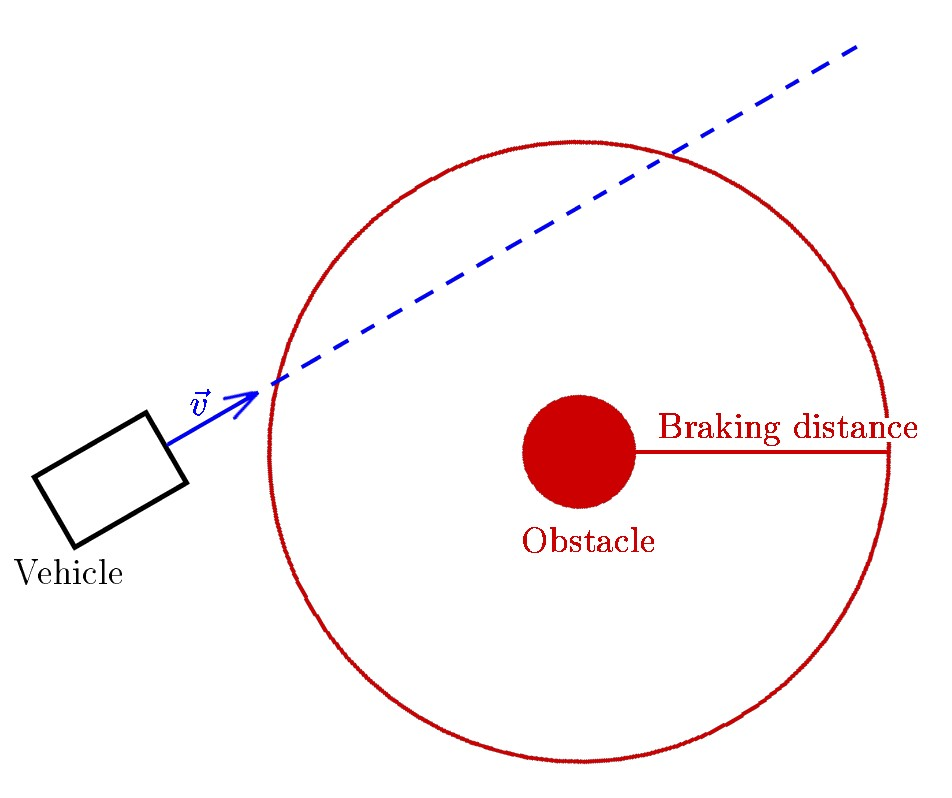
\includegraphics[height=8cm]{trajectory.jpg}
\caption{A safe but unacceptable trajectory}\label{OA}
\end{center}
\end{figure}

\subsection{Physical model and hypothesis}

We assume that the obstacle is fixed and given by its absolute position (GPS coordinates), and the vehicles sensors also give its absolute position.
Operator commands are given by an absolute speed (direction and velocity) to set to the vehicle, which should be either accepted or causing the vehicle to stop to stay at a minimal safe distance $D$ of the obstacle.
If the vehicle is already below this safe distance, we should only accept command that take the vehicle away from the obstacle.

The system could be represented as follows: A sensor node communicates the position to the controller through a $\mathit{Input}$ topic, and the controller node sends commands to the engine to set the new speed with the $Output$ topic. 
The controller node is also responsible for the communication with the operator. %(see Figure \ref{...})
For more simplicity, we model this link by a variable \texttt{OpCommand}, accessible by the controller and supposed to be updated each time a new command is received from the operator.

% Add beautiful schema here

We assume there is a known function $b(v)$ that, for a velocity $v$, gives the distance used to stop completely from the moment the vehicle begins to brake\footnote{$ $
In case the vehicle purposely doesn't brake at full power when the speed is too high to avoid tilting}.
In other cases, we assume that the new speed is set immediately after the command is computed by the engine node (in usual conditions, commands given by an operator -- that are not "stop!" -- are small variations of the current speed).
This would only add complexity to the explanations, but not change fundamentally the ideas presented here, so we assume the position is known exactly, and that the speed after a computation of the engine is exactly the speed contained in the received command.
Finally, we assume the parameters of the $Output$ topic are chosen in such a way that the message order is preserved.

\subsection{Controller strategy}

We use the same notations as in section~\ref{MAdef}, except for the engine node noted $E$ and its execution noted $e(n)$.
Because the system is asynchronous, when the controller receives a position from the sensor, the actual position may have changed depending on previous set speeds.
We also need to consider the potential delay before a command issued by the controller is executed by the engine.

We assume the controller keeps a buffer of the $N$ previous set speeds with
\[N = \left\lceil \frac{MA(Input) + MA(Output) + maxT(E)}{minT(C)} \right\rceil\]
Initially, this buffer is filled with zeros and each time a command is sent, the corresponding speed is added at the end of the buffer (after removing the first value).

This way, the buffer contains at time $t$ all speeds that were sent from $t - \big ( MA(Input) + MA(Output) + maxT(E) \big )$ to $t$. So, assume the controller executes $c(n)$ and $s(k)$ is the sensor message that is used, then for all time $t$ in $[s(k), c(n)]$, the actual speed at time $t$ is contained in the buffer.
We assumed $Output$ preserves the message order, so for $t$ in $[c(n), e(l)]$ (where $e(l)$ is a step of the engine that uses $c(n)$), the actual speed at time $t$ is in the updated buffer.

\paragraph{ }For each speed $\vec{v} = v.\vec{u}$ in the buffer and in the variable \texttt{OpCommand}, we compute the set of positions $Unsafe(\vec{v})$ that are at a distance less than $b(v)$ in the direction $\vec{u}$ from the unsafe zone\footnote{i.e. the points at a distance less than $D$ to the obstacle, assumed to be the origin}:
\[Unsafe(\vec{v}) = \Big \{ P \,| \, \exists d \leq b(v), \, \| P + d.\vec{u} \| \leq D \Big \} \]

Then, we extend this zone considering the buffered speeds and the new desired speed. More precisely, we consider the positions from which we can get in $Unsafe(\vec{v})$ using some composition of these speeds in less than $\lambda = MA(Input) + MA(Output) + maxT(E)$. 
Formally, let \mbox{$(\vec{v_1}, \dots, \vec{v_n})$} be the buffer, and $\vec{v_0}$ the speed contained in \texttt{OpCommand}. Then, the extended zone is:
\[Unsafe_{ext}(\vec{v}) = \left\{ P \,| \quad
\exists t_0, \dots, t_n, \quad \sum_{i=0}^N t_i \leq \lambda \, \textrm{ and } \,
P + \sum_{i=0}^N t_i.\vec{v_i} \in Unsafe(\vec{v}) \right\} \]

If the measured position is inside one of the $Unsafe_{ext}(\vec{v_i})$, the vehicle should stop, so the controller sends a command containing a zero speed. Otherwise, it is safe to proceed the user's instruction.
In both cases, the buffer must be actualized.


\subsection{Elements of correctness proof}

The main argument is quite simple: the vehicle runs into the obstacle if it doesn't brake soon enough, that is, at some point, the vehicle has a speed $\vec{v}$, is in $Unsafe(\vec{v})$ and is not braking.
With said strategy, this is not possible.

Assume at time $T$, the vehicle is in this situation. The speed was set during a computation $e(n)$ of the engine according to a command $c(k)$ from the controller.
When $c(k)$ occurred, we had $\texttt{OpCommand} = \vec{v}$ ($\vec{v} \neq \vec{0}$ is the command that was sent), and let $B$ be the state of the buffer at this point (before update).
The controller made the decision to send the command $\vec{v}$ according to this speed, the buffer state $B$, and a position measured at $s(l)$; and (among others) $s(l) \notin Unsafe_{ext}(\vec{v})$ -- otherwise the controller would have sent the stop order.

We know by definition of the buffer that for $t \in [s(l), c(k)]$, the speed at time $t$ was in $B$,
and for $t \in [c(k), e(n)]$, the speed at time $t$ was in the updated buffer. Also, for $t \in [e(n), T]$, the speed was $\vec{v}$. 
In each case, the speed was in $B \bigcup \{ \vec{v} \}$.
By definition of these bounds, we have $T - e(n) \leq maxT(E)$, $e(n) - c(k) \leq MA(Output)$ and $c(k) - s(l) \leq MA(Input)$.
This means the vehicle went from outside $Unsafe_{ext}(\vec{v})$ to inside $Unsafe(\vec{v})$ in less than $\lambda$, which is impossible by assumption.


\subsection{Future work}

Unlike properties given in Sections 4 to 6, this result has not been formally proved with PVS, so such an implementation is a first possible extension.
However, the proof needs first to be completed before being mechanically verified: an identified gap is the influence of zero speeds added to the buffer when the \emph{stop} command is sent.
Actually, the assumption is that for all $t$ in some past time interval, the speed at time $t$ is in the buffer, but (unlike non-zero speeds) when a zero speed is processed by the engine, the speed is not set to 0 immediately because of the braking distance.
This could be solved by more assumptions on the engine node; for example, when the \emph{stop} command is processed, all other commands are ignored until the vehicle has come to full stop, plus some delay to cover communication latency.

Also, it could be helpful to find linear approximations of used sets (especially $Unsafe_{ext}(\vec{v})$) in order to reduce computing time. 
Another direction could be to replace the speed buffer by a measured value and dynamic properties of the vehicle (acceleration power / direction change capabilities).
This would give a more realistic physical model, but it would need a more complex analysis to ensures the vehicle responds to operator commands.










\bibliographystyle{plain}
\bibliography{biblio}


\end{document}
